\documentclass[10pt,a4paper]{article}
\usepackage[english]{babel}
\usepackage[utf8]{inputenc}
\usepackage{amsmath}
\usepackage{amsfonts}
\usepackage{amssymb}
\usepackage{graphicx}
\usepackage{float}
\usepackage{caption}

%< > ... dummy content zur Veranschaulichung

\begin{document}
	\part*{Model Documentation of the \\ Kapitza's Pendulum} % MUST - Add Model Name 
	
	%%%%%%%%%%%%%%%%%%%%%% NOMENCLATURE %%%%%%%%%%%%%%%%%%%%%%%%%%%
	
	\section{Nomenclature} % MUST
	\subsection{Nomenclature for Model Equations} % MUST
	
	%variables for model equations
	\begin{tabular}{ll}
		$\gamma$ & Dampening factor \\
		$l$ & length of the pendulum \\
		$g$ & acceleration due to gravity \\
		$\varphi$ & angle of deflection from the equilibrium position \\
		$a$ & magnitude of the harmonic oscillation of the suspension point \\
		$\omega$ & frequency of the harmonic oscillation of the suspension point
				
	\end{tabular}
	 
	
	\subsection{Graphic of the Structure}	
	\begin{figure}[H]
		\centering
		\captionsetup{justification=centering, margin=1cm}
		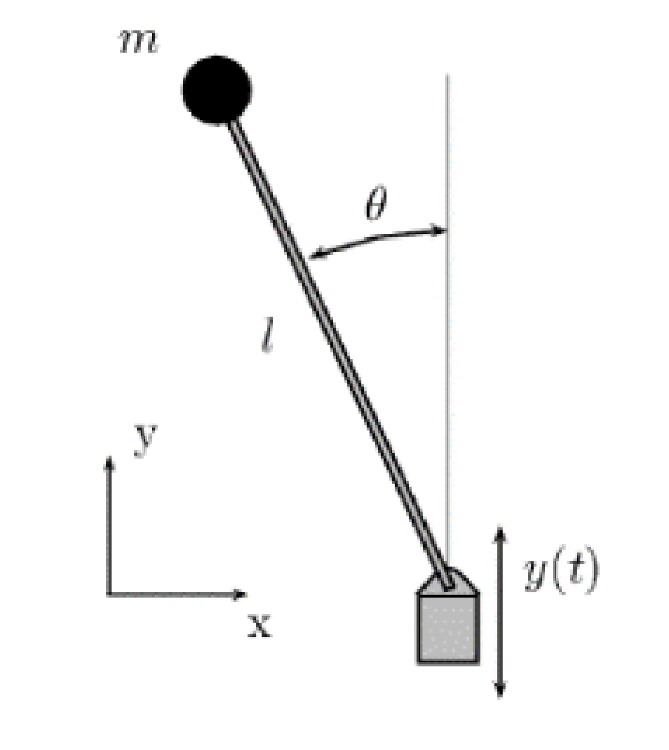
\includegraphics[width=45mm]{kapitza_pendulum.pdf}
		\caption{Structure of the Pendulum. \\ \footnotesize{Source: Bello, Thomas; Huang, Emily; Lopez, Fabian; Rumsey, Kellin; Tao, Tao / Pendulum With Vibrating Base}}
	\end{figure}
	
	%%%%%%%%%%%%%%%%%%%%%% MDOEL EQUATIONS %%%%%%%%%%%%%%%%%%%%%%%%%%%
	
	\section{Model Equations} % MUST
	
	State Vector and Input Vector:
	\begin{align*}
		\underline{x} &= (x_1 \ x_2)^T = (\varphi \ \dot{\varphi})^T \\
		\underline{u} &= \emptyset
	\end{align*}
	
	\noindent System Equations:			
	\begin{subequations}
	\begin{align}
		\dot{x}_1 &= x_2 \\
		\dot{x}_2 &= -2\gamma x_2 - \left(\frac{g}{l} - \frac{a}{l}\omega^2\cos(\omega t)\right)\sin(x_1)
	\end{align}
	\end{subequations}

	%%%%%%%%%%%%%%%%%%%%%% PARAMETERS | OUTPUTS %%%%%%%%%%%%%%%%%%%%%%%%%%%
	\noindent
	Parameters: $\omega, ~a, ~l, ~g, ~\gamma$ % variables with constant, predefined value
	\\
	Outputs: $\varphi$ % MAY
	
	%%%%%%%%%%%%%%%%%%%%%% ASSUMPTIONS %%%%%%%%%%%%%%%%%%%%%%%%%%%
	
	\subsection{Assumptions} % MAY 
		\begin{enumerate} %possible list type for the Assumptions - mögliche Formatierung für die Annahmen
			\item Mass of the pendulum is a pointmass. 
		\end{enumerate}
	
	%%%%%%%%%%%%%%%%%%%%%% EXEMPLARY PARAMETER VALUES %%%%%%%%%%%%%%%%%%%%%%%%%%%	
	
	\subsection{Exemplary parameter values}
	\begin{tabular}{cl}
\hline
  Symbol  & Value                                                                                                                                                                                \\
\hline
   $A$    & $\left[\begin{matrix}0.8189 & 0.0863 & 0.09 & 0.0813\\0.2524 & 1.0033 & 0.0313 & 0.2004\\-0.0545 & 0.0102 & 0.7901 & -0.258\\-0.1918 & -0.1034 & 0.1602 & 0.8604\end{matrix}\right]$ \\
   $B$    & $\left[\begin{matrix}0.0045 & 0.0044\\0.1001 & 0.01\\0.0003 & -0.0136\\-0.0051 & 0.0936\end{matrix}\right]$                                                                          \\
 $B_{1}$  & $\left[\begin{matrix}0.0045 & 0.0044\\0.1001 & 0.01\\0.0003 & -0.0136\\-0.0051 & 0.0936\end{matrix}\right]$                                                                          \\
 $C_{1}$  & $\left[\begin{matrix}1.0 & 0 & -1.0 & 0\\0 & 0 & 0 & 0\\0 & 0 & 0 & 0\end{matrix}\right]$                                                                                            \\
   $C$    & $\left[\begin{matrix}1.0 & 0 & 0 & 0\\0 & 0 & 1.0 & 0\end{matrix}\right]$                                                                                                            \\
 $D_{11}$ & $\left[\begin{matrix}0 & 0 & 0\\0 & 0 & 0\\0 & 0 & 0\end{matrix}\right]$                                                                                                             \\
 $D_{12}$ & $\left[\begin{matrix}0 & 0\\1.0 & 0\\0 & 1.0\end{matrix}\right]$                                                                                                                     \\
 $D_{21}$ & $\left[\begin{matrix}0 & 1.0 & 0\\0 & 0 & 1.0\end{matrix}\right]$                                                                                                                    \\
\hline
\end{tabular}
%	\begin{tabular}{lcl} 
%		Parameter & Symbol & Value \\ \hline
%		Pendulum length & l & 10cm \\
%		Amplitude of Oscillation & a & 2cm \\
%		Frequency of Oscillation & $\omega$ & $16\omega_0$ \\
%		Dampening Factor & $\gamma$ & $0.1\omega_0$
%	\end{tabular}
	\\
	with $\omega_0$ = $\sqrt{\frac{g}{l}}$

	%%%%%%%%%%%%%%%%%%%%%% DERIVATION & EXPLANATION %%%%%%%%%%%%%%%%%%%%%%%%%%%	
	
	\section{Derivation and Explanation} % SHOULD
	The Lagrangian mechanics was used for the solution.
	
	%%%%%%%%%%%%%%%%%%%%%% REFERENCES %%%%%%%%%%%%%%%%%%%%%%%%%%%
	
	\begin{thebibliography}{10}		
		\bibitem{But21}Butikov, E. I.: 
		\textit{Kapitza’s Pendulum: A Physically Transparent Simple Treatment}, published 2017.
		\bibitem{Fig1}Bello, Thomas; Huang, Emily; Lopez, Fabian; Rumsey, Kellin; Tao Tao: 
		\textit{Pendulum With Vibrating Base}, published 2014.
	\end{thebibliography}	
		

\end{document}